\documentclass[conference,compsoc]{IEEEtran}

\usepackage[utf8]{inputenc}
\usepackage[spanish]{babel}
\usepackage{babelbib}
\usepackage{tikz}
\usepackage{listings}
\usepackage{soul}
\usepackage{graphicx}
\usepackage{float}

\renewcommand\IEEEkeywordsname{Palabras clave}

\begin{document}

\title{Aplicación del algoritmo Kmeans con la plataforma Spark}

\author{
    \IEEEauthorblockN{Carlos Andres Sanchez Alzate}
    \IEEEauthorblockA{
        Universidad EAFIT\\
        csanch35@eafit.edu.co
    }
    \and
    \IEEEauthorblockN{Alejandro Salgado Gómez}
    \IEEEauthorblockA{
        Universidad EAFIT\\
        asalgad2@eafit.edu.co
    }
}

\maketitle

\begin{IEEEkeywords}
    Kmeans, Spark, Big data, TF-IDF
\end{IEEEkeywords}

\vspace{0.5cm}

\begin{abstract}
Las nuevas técnologías traen consigo cambios en la forma realizar las labores
de creación de algoritmos pues debido a la cantidad de información que
producimos para representar el mundo real en entornos virtuales, hace generar
la imperiosa necesidad de acelerar el crecimiento de los atributos o cualidades
del hardware de las máquinas que producimos. A pesar de que las tecnologías de
paralelización existen ya hace algunos años, con este crecimiento abrumador de
la información que producimos, nos vemos en la obligación de migrar a un
razonamiento en paralelo respecto a la producción de algoritmos. En este
articulo veremos como la programación paralela efecta la solución del problema
respecto al timpo de respuesta que esta nos brinda, tomando como base un
problema cotidiano como lo es el procesamiento del lenguaje natural y la
minería de datos para la clasificación de libros.
\end{abstract}

\section{Introducción}
Muchos de los datos que encontramos en la web, están dispuestos en forma de
texto y generalmente están allí  con el proposito de informar o expresar ideas
y difundir información de una forma más efectiva. Entender o descifrar  el
significado de las símobolos plasmados en textos es una caracteristica de los
humanos, pero con el auge de la producción masiva de información que conlleva
al crecimiento de la producción textual por medios digitales, carecemos de la
habilidad de procesar cientos o miles de ellos para llevar a cabo tareas más
complejas como la clasificación en un tiempo razonable.\\

Para las máquinas también se dificulta esta tarea cuando la cantidad de
información que se procesa es muy grande, puesto que estás también tienen
recursos limitados y para aprovechar al máximo el uso de estos recursos debemos
conocer muy bien la arquitectura que poseen, pues estás actualmente cuentan con
la capacidad de procesar información en paralelo, caracteristica que nos
permite disminuir el tiempo de computo y completar de forma más rápida las
tareas que pretendemos realizar.\\

En este ariticulo se explicará y analizará una metodología para la optimización
de un algoritmo de clasificación de textos y como elaboramos un modelo que nos
permita representar de forma adecuada los texto que se desean clasificar. El
objetivo de este trabajo es utilizar técnicas de análisis sobre grandes
volumenes de información para lograr el objetivo planteado anteriormente.

\section{Descripción del problema}

En la actualidad el NPL (Natural Processing Language), es una área de estudio
que ha cobrado mucha importancia para el procesamiento y entendimiento del
leguaje natural realizado de forma automática, esto ha permitido dotar a las
máquinas de la capacidad de ejecutar tareas complejas que serían dificiles o
imposibles de realizar por el ser humano.\\

La clasificación en la minería de datos es uno los problemas usados para la
exploración de soluciones en divesos problemas de manipualción de textos, estas
técnicas nos dotan de la capacidad de categorizar y detectar similaridades
entre grupos de datos para organizarlos bajo criterios de distancias entre cada
uno de sus elementos, y cuyos componentes se relacionan entre si por su
cercanía, de modo que al agruparlos bajo este criterio podemos generar
subgrupos donde sus elementos aducen caracteristicas similares, asi se puede
identificar con mayor facilidad peculiaridades generales de los datos que
analizamos.\\

\subsection{TF-IDF}
Para la extracción de características de los documentos, en este trabajo se
utilizará la implementación del algoritmo de TF-IDF para representar los textos
numéricamente a partir de palabras que los conforman. TF-IDF tiene diversas
aplicaciones, entre ellas están el reconocimiento de patrones y la
clasificación de documentos, bajo este último enfoque, es un método que es
usado para representar documentos ignorando su gramática y el orden de las
palabras, este algoritmo logra obtener información sobre la importancia de los
terminos que componen un documento.\\

TF-IDF nos permite generar una reprecentación numérica a partir de textos con
las cuales podemos utilizar como entrada a diversos algoritmos de
clasificación, por ejemplo kmeans. Dichas representaciones son generadas a
partir de una funcion hash, la cual es usada para obtener una primera
representación del documento y posteriormente es utilizada para priorizar los
terminos del texto.\\

\subsection{K-Means}
En términos generales, clustering tiene como objetivo dividir un conjunto
determinado de objetos en grupos, de modo que los objetos en el mismo grupo
sean similares y los objetos en diferentes grupos sean diferentes entre sí. El
término objetos se usa para referirse a entidades, observaciones o puntos de
datos en un conjunto de datos. El término clúster, aunque no tiene una
definición precisa este describe un grupo de objetos.\\

El clustering con K-means es un algoritmo de clasificación y un técnica de
entrenamiento no supervidada, y es el mejor representante del clustering duro
(No difuso). Por clústeres duro nos referimos a los algoritmos de clustering
que intentan dividir los datos disponibles en algunos subconjuntos para que
cada punto de datos solo puede pertenecer a un subconjunto.\\

En particular, K-means tiene como objetivo dividir un conjunto de n puntos de
datos x1, x2,... , xn en K clusters C1, C2,. . . , CK tal que la función de
costo J se minimiza:

\begin{figure}[H]
    \centering
    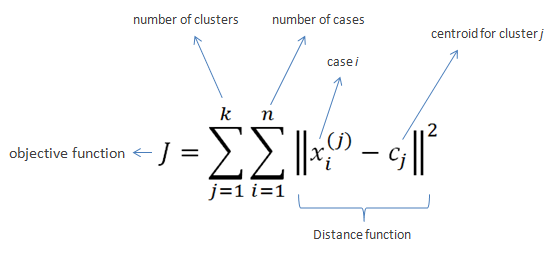
\includegraphics[scale=0.6]{kmeans.png}
    \caption{Función objetivo del algoritmo Kmeans} \cite{kmeans}
\end{figure}

En el conjunto de observaciones x1, x2, ..., xn, cada observación es un vector
real con d dimensiones, el algoritmo construye k subconjuntos de las
observaciones con el fin de minimizar la suma de cuadrados dentro de cada
grupo.\\

Para la implementación de k means se pueden usar diferentes criterios de medida
para calcular las distancias de los puntos a los centroides, en particular en
la ecuación 1, se hizo uso de la distancia euclideana y está será la que
seguiremos utilizando en este trabajo.

Abajo detallaremos un algoritmo básico de K-means, el cual consta de 5 pasos.\\

\begin{enumerate}[]
    \item Seleccione aleatoriamente K puntos de datos del conjunto de datos de
          entrada y asignelos como centroides de los clústeres c1, c2,..., cK.
    \item Calculamos la distancia entre los centroides y cada uno de los datos.
    \item Calculamos la posición de los centroides de modo que estos se ubiquen
          aproximadamente en el centro del cluster.
    \item Repetimos del el paso 2 y 4 hasta cumplir con los criterios de parada
          que se definan.\\

Este algortimo de clustering puede ayudarnos a revelar la estructura subyacente
de los datos y, por este motivo,se ha convertido en una de las técnicas más
utilizadas para el análisis exploratorio de datos en diferentes campos de la
ciencia y la ingeniería.

\end{enumerate}

\section{Análisis y diseño}

Para la implementacion del algoritmo se tuvieron en cuenta varios factores,
el primero de ellos fue la forma de represantar los textos de tal manera que se
les pueda calcular una medida de distancia. Para lograr este objetivo es
necesario representarlos de forma numérica, por ello se hacía necesario el uso
de un algoritmo que nos permitiera traducir los textos en vecotres de
carácteristicas sobre los cuales se pudieran efectuar
operaciones matematicas. Despues de analizar varias alternativas, se decidió
utilizar el algoritmo TF-IDF.\\

TF-IDF es un algoritmo compuesto por 4 etapas, la primera de ellas es la
representación de los documentos en una primera version numérica, para esto
se utiliza una función hash.

\begin{figure}[H]
    \centering
    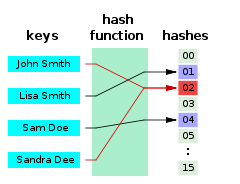
\includegraphics[scale=0.6]{hash.png}
    \caption{Función hash} \cite{hash}
\end{figure}

Dicha función toma las palabras de cada uno de los textos y devuelve un
identificador numerico que la representa. Luego esta representación es usada
para calcular la frecuencia de las palabras en el texto, esta etapa es llamada
TF (Term frequency). Es necesario tener en cuenta que debido a la manera en la
que opera una función hash pueden presentarce colisiones, lo que siginifica
que dos palabras distintas puedan ser asignadas al mismo numero, para disminuir
este problema se puede aumentar el rango de la función, en este caso
se utilizó $2^{20}$, el cual es el estandar de la libreria de machine learning
de Spark.\\

Posteriormente se calcula la importancia de cada una de las palabras basados en
el siguiente modelo\\

\begin{equation}
    IDF(t,D) = log \left( \frac{|D| + 1}{DF(t,D) + 1} \right)
\end{equation}

\vspace{0.5cm}

Donde $D$ es el conjunto de documentos a ser analizados, $t$ representa el
termino al que se le desea calcular su importancia, $|D|$ representa la
cardinalidad del conjunto $D$, es decir la cantidad de documentos, y $DF(t,D)$
representa la cantidad de documentos en la que el termino en cuestión aperece.\\

Para entender mejor la forma de esta función es necesario recordar ciertos aspectos,
el primero de ellos es que una división no esta definida si su denominador es $0$,
por esta razón se debe agregar un $1$ al cálculo de la función $DF(t,D)$ para asegurar
que la división siempre este definida. En segundo lugar se debe recordar que el
logaritmo se anula en $x=0$, tal como se muestra en la Figura \ref{fun:log}, lo que
explica la adición de una unidad al cálculo del numerador para evitar que la función
$IDF(t,D)$ resulte en un valor nulo. Finalmente es necesario notar que la
desigualdad $|D| >= DF(t,D)$ siempre es verdad, lo que implica que la división
tiene el dominio $[1,\infty)$, tal como se muestra en la Figura \ref{fun:logpos},
lo que significa que la expresion trabajada siempre resultara en valores positivos,
los cuales son acotados por la función logaritmo.

\begin{figure}[H]
    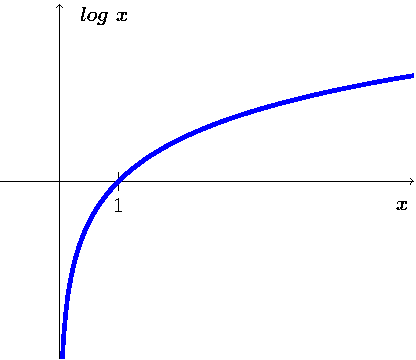
\includegraphics[scale=1]{Logarithm.pdf}
    \caption{Función logaritmo}
    \label{fun:log}
\end{figure}

Una vez entendido esto se puede observar como la funcion $IDF(t,D)$ provee información
sobre la importancia de un termino, esto se debe a que tiene en cuenta la relación entre
la cantidad de documentos que contienen el termino en cuestion con la cantidad de
documentos totales, lo que implica que los terminos que son bastante repetidos tendran
una importancia baja, resultando en una influencia baja en la decision de clasificación,
mientras que los terminos más unicos seran clasificados con un valor más alto, implicando
que tendran una importancia mayor en la etapa de clasificación.

\begin{figure}[H]
    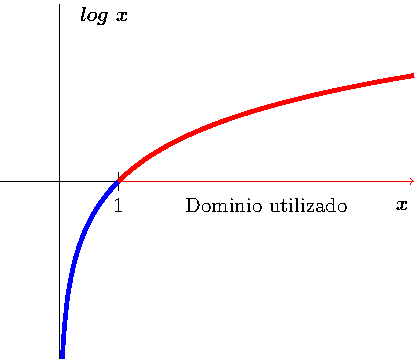
\includegraphics[scale=1]{LogarithmPos.pdf}
    \caption{Parte usada de la función logaritmo}
    \label{fun:logpos}
\end{figure}

Finalmente la clasificación total de los terminos es calculada como la multiplicación
entre el factor $TF$ y $IDF$ para asociar tanto la cantidad de veces que un termino
aparece en el texto, como su importancia general, obteniendo así la representación
numerica final que sera usada como entrada para el algoritmo Kmeans.\\

Ahora, en cuanto al rendimiento de esta nueva implementación, se espera que
los tiempos necesarios para completar la ejecución sean mayores que la version realizada
en el proyecto pasado, esto por varias razones, la primera es la plataforma de ejecución,
debido a que en la practica de HPC se utilizaba el hardware directamente desde
la aplicación, el rendimiento podia subir más de lo que se podria lograr con las
maquinas virtuales del cluster Hadoop, incluso teniendo en cuenta que en esta
ultima plataforma se hacia uso de una arquitectura distribuida. En segundo lugar
el el lenguaje de programación, en la practica pasada se utilizo C++ con Cuda para
implementar el algoritmo, mientras que en este proyecto se utilizo Python, lo que
agrega capas de abstracción, las cuales facilitan la programación, pero aumentan
los tiempos de ejecución. Finalmente tal como se hablo en la practica pasada,
se encontro que una implementación en GPU resulta en menores tiempos de ejecución
gracias a su arquitectura altamente paralela y su rapida creación de procesos.\\

Sin embargo, una implementación como la que se presenta en esta practica no siempre
tendra un rendimiento menor a una diseñada para ejecutar en un ambiente HPC, de
hecho es necesario que estos algoritmos puedan ser implementados en arquitecturas
diseñadas para el tratamiento de grandes volumenes de datos, tal como un cluster
Hadoop, debido a que, apesar de su velocidad, una infraestructura HPC perderia
gran parte de su rendimiento en casos en los que la cantidad de datos sea grande,
mientras que arquitecturas como la utilizada en este proyecto mostrarian todo
su potencial logrando tiempos de ejecucion y costos mucho menores. Por esta razón
es necesario hacer la aclaración de que se espera un rendimiento menor que en la
practica de HPC, pero esto se debe al tamaño de los datos utilizados.

\section{Implementación}

Teniendo en cuenta que se trata un problema en el cúal puede estar involucrado
el procesamiento de granades volumens de información, se hace uso de
herramientas diseñadas especialmente para este proposito, como lo son Apache
Spark y Hdfs del ecosistema Hadoop, quienes son utilizados respectivamente para
el procesamiento de la información y su almacenamiento.\\

para la clasifiación de los documentos, se hace uso de las librerías que provee
Spark, de las cuales algunas de las funciones implementadas están diseñadas
para este proposito. apache spark posee funciones para la transformación de los
docuementos en representaciones numéricas o cuantitavas, en este trabajo se
hace uso de TF e IDF, las cuales realizan el procesaminto de los archivos de
textos como se explicó en la sección de analisis y diseño. Después de la
transformación de los documentos se procede a utilizar kmeans, la cúal se
encuentra implementada en la libreria Mlib de Apache Spark.\\

Para la tranfoamción del documento en una correcta representación numérica para
claificar los docuemntos con Kmeans se requiere utilizar dos funciones que
Spark provee de forma independiente, las cuales son TF e IDF.\\

la función tf calcula la frecuencia de las palabras dentro del documento, a
esta se le debe pasar como parametro el documento que queremos transformar y lo
hacemos de la siguente manera.\\

\begin{lstlisting}
    tf = hashingTF.transform(documents)
\end{lstlisting}

\vspace{0.5cm}

Luego procedemos a calcular los valores de la frecuencua inversa de las
palabras de los documentos, la cual nos permite conocer la importancia de las
palabras en esto. A esta función le pasamos como parametro la variable tf, la
cual calculas con anterioridad.\\

\begin{lstlisting}
    idf = IDF(minDocFreq=5).fit(tf)
\end{lstlisting}

\vspace{0.5cm}

Para terminar con la transformación debemos multiplicar td e idf, y dicho valor
nos dará los valores finales de la importancia de cada las palabras dentro de
los documentos.

\section{Resultados}

\begin{figure}[H]
    \centering
    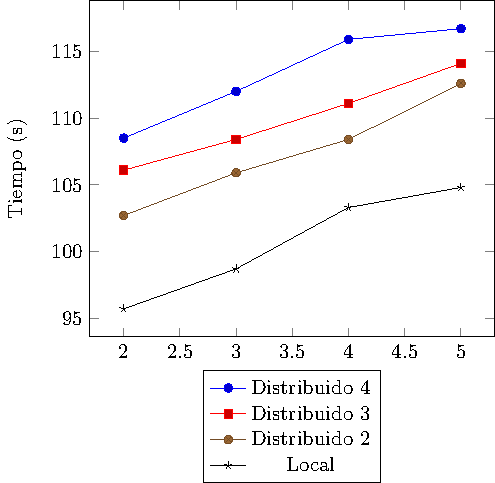
\includegraphics[scale=1]{ResultsSpark.pdf}
    \caption{Resultados Spark}
\end{figure}

\begin{figure}[H]
    \centering
    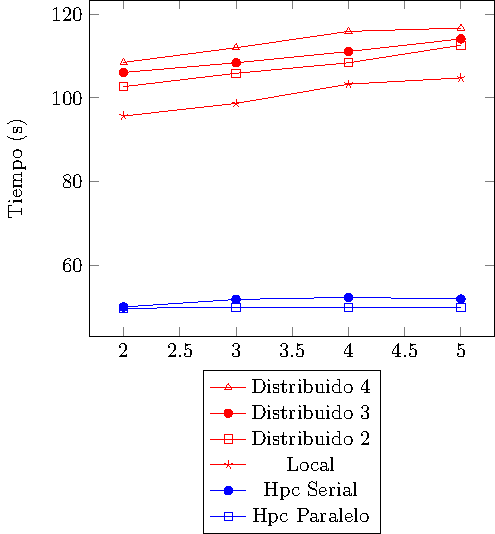
\includegraphics[scale=1]{ResultsCombined.pdf}
    \caption{Resultados combinados}
\end{figure}

\section{Conclusiones}


\bibliographystyle{unsrt}
\bibliography{Documentation}

\end{document}
